\textbf{COLUNI 2026 -- Questão 24}\par\medskip A placa ilustrada na figura a seguir é constituída por um material que tem sua massa distribuída homogeneamente. Ela é sustentada por dois cabos A e B de massas desprezíveis. A placa excede a marquise que a sustenta, como ilustrado na figura a seguir.

\begin{figure}[htbp]
\centering
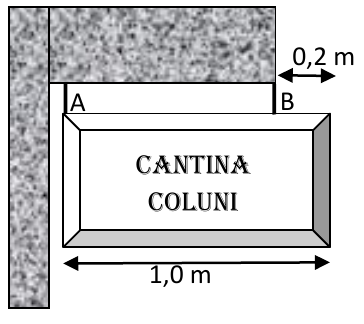
\includegraphics[width=0.56\linewidth]{static/simulados/coluni/figuras/2026/questao-24/figura-2.png}
\end{figure}

Comparando as intensidades das forças tensoras, $T_A$ e $T_B$, nos cabos A e B, é CORRETO afirmar que:\begin{enumerate}
\item $T_A=1{,}0\,T_B$
\item $T_A=0{,}6\,T_B$
\item $T_A=0{,}3\,T_B$
\item $T_A=0{,}5\,T_B$\end{enumerate}